\documentclass[sigconf,nonacm]{acmart}

\usepackage{xcolor}
\usepackage{graphicx}
\usepackage{booktabs}
\graphicspath{{figures/}}

\title[Traffic Accident Spillovers]{Causal Graph Learning for Traffic Accident Spillovers}
\subtitle{{Midpoint Progress Report}}

\author{Kyle Luong}
\authornote{All authors contributed equally to this work.}
\email{auj7tx@virginia.edu}
\affiliation{\institution{University of Virginia}\city{Charlottesville}\state{Virginia}\country{USA}}

\author{Nate Mackintosh}
\authornotemark[1]
\email{qjz5my@virginia.edu}
\affiliation{\institution{University of Virginia}\city{Charlottesville}\state{Virginia}\country{USA}}

\author{Maddox Shrum}
\authornotemark[1]
\email{tyq3jy@virginia.edu}
\affiliation{\institution{University of Virginia}\city{Charlottesville}\state{Virginia}\country{USA}}

\renewcommand{\shortauthors}{Luong et al.}

\begin{document}

\begin{abstract}
Traffic accidents can slow traffic on the incident road and on connected
roads. We propose a causal graph learning study of these effects using
Chicago crash reports and historical traffic speeds. We will compare
matched event studies with graph-based counterfactual models to estimate
how slowdowns change across roads and time. Our goal is to test whether
network learning improves \emph{causal effect estimation}, not only
traffic prediction.

{For this midpoint review, we report an integrated
pipeline using March--April 2025 data: 2{,}529 eligible crash events,
a graph of 879 monitored road segments, and three trained forecasting
models. Preliminary matched-control results suggest modest speed
reductions on crash segments. The analysis supports further study of
spillovers, but does not yet establish causal effects or a benefit
from graph learning.}
\end{abstract}

\keywords{graph machine learning, causal inference, traffic accidents,
spatiotemporal graphs, network interference}
\maketitle

\section{Research Direction}
An accident may disrupt traffic on several connected roads. Its effect
depends on the road network and on traffic conditions before the event.
We study this as a problem of \emph{network interference}: an event at
one segment may change outcomes at other segments.

\noindent\textbf{Main question:} Can graph learning improve estimates
of the traffic slowdowns caused by accidents, including their spread
across connected roads over time?

\section{Related Work}
Cao et al. estimate incident-related speed reductions and identify
spatiotemporal regions affected by incidents \cite{cao2021traffic}.
Li et al. use doubly robust causal learning to estimate how crash
effects vary across highway locations and conditions
\cite{li2024crash}. These studies show why comparing raw before-and-after
speeds is insufficient.

CASTANET combines graph learning and causal effect estimates to
forecast traffic after incidents \cite{kitahara2026castanet}.
Our focus is more specific: whether road-network information improves
\emph{estimation of the effects themselves}, particularly on roads
that do not experience the crash. CASTANET emphasizes incident-aware
forecasting; our study will separately evaluate counterfactual quality
and causal evidence. Using a GNN alone is not our proposed contribution.

\section{Problem and Data}
\begin{itemize}
    \item \textbf{Graph:} Nodes are monitored road segments; edges
    represent road connections. Direction will be used where reliable.
    \item \textbf{Exposure:} A reported accident on one segment.
    Connected segments may experience indirect exposure.
    \item \textbf{Outcome:} Segment-level traffic speed before and
    after the accident.
    \item \textbf{Causal target:} Speed differences attributable to
    the accident, relative to comparable conditions without it.
\end{itemize}

Chicago publishes crash times and locations and ten-minute arterial
speed estimates \cite{chicagoCrashes,chicagoSpeeds}. The speed series
uses bus GPS data and ends in April 2026
\cite{chicagoTrackerNotice}. It does not cover every road. We will
first check crash-to-segment matches, timestamp quality, and speed
coverage on a small connected network before fixing the sample.


% BEGIN MIDPOINT ADDITION: pilot implementation and findings (red)
\section{{Midpoint Progress}}
{We evaluated March 1--April 30, 2025, using ten-minute
intervals, two hours of historical speeds, and a one-hour forecast
horizon. The results below are from a single run (seed 42); the
experiment settings and code revision are saved with the outputs.}

\subsection{{Data and Network Feasibility}}
{Table~\ref{tab:midpoint_funnel} summarizes sample
selection. Of 17{,}658 reported crashes, 3{,}668 could be matched to
monitored road segments. This reduction largely reflects the limited
coverage of arterial speed measurements. After applying pre-event
history and matched-control requirements, 2{,}529 crashes remain for
the preliminary analysis. The 297 events with complete pre- and
post-event observations form a stricter subset, not the main sample.}

\begin{table}[t]
\centering
\caption{{Crash sample, March--April 2025. Retention
is relative to all reported crashes.}}
\label{tab:midpoint_funnel}
\footnotesize
{\begin{tabular}{lrr}
\toprule
Stage & Crashes & Retained \\
\midrule
All reported crashes & 17{,}658 & 100.0\% \\
Valid coordinates & 17{,}479 & 99.0\% \\
Matched monitored road & 3{,}668 & 20.8\% \\
Window within speed history & 3{,}666 & 20.8\% \\
\textbf{Analysis sample} & \textbf{2{,}529} & \textbf{14.3\%} \\
\quad Complete-case subset & 297 & 1.7\% \\
\bottomrule
\end{tabular}}
\end{table}

{Speed measurements are available for 53.8\% of
road--time cells. We retain partially observed windows and mask
missing outcomes rather than treating missing speeds as zero. The
modeling graph has 879 speed-observed segments and 4{,}726 edges;
795 segments (90.4\%) belong to its largest connected component.}

\begin{figure}[t]
\centering
\IfFileExists{figures/road_network.png}{%
  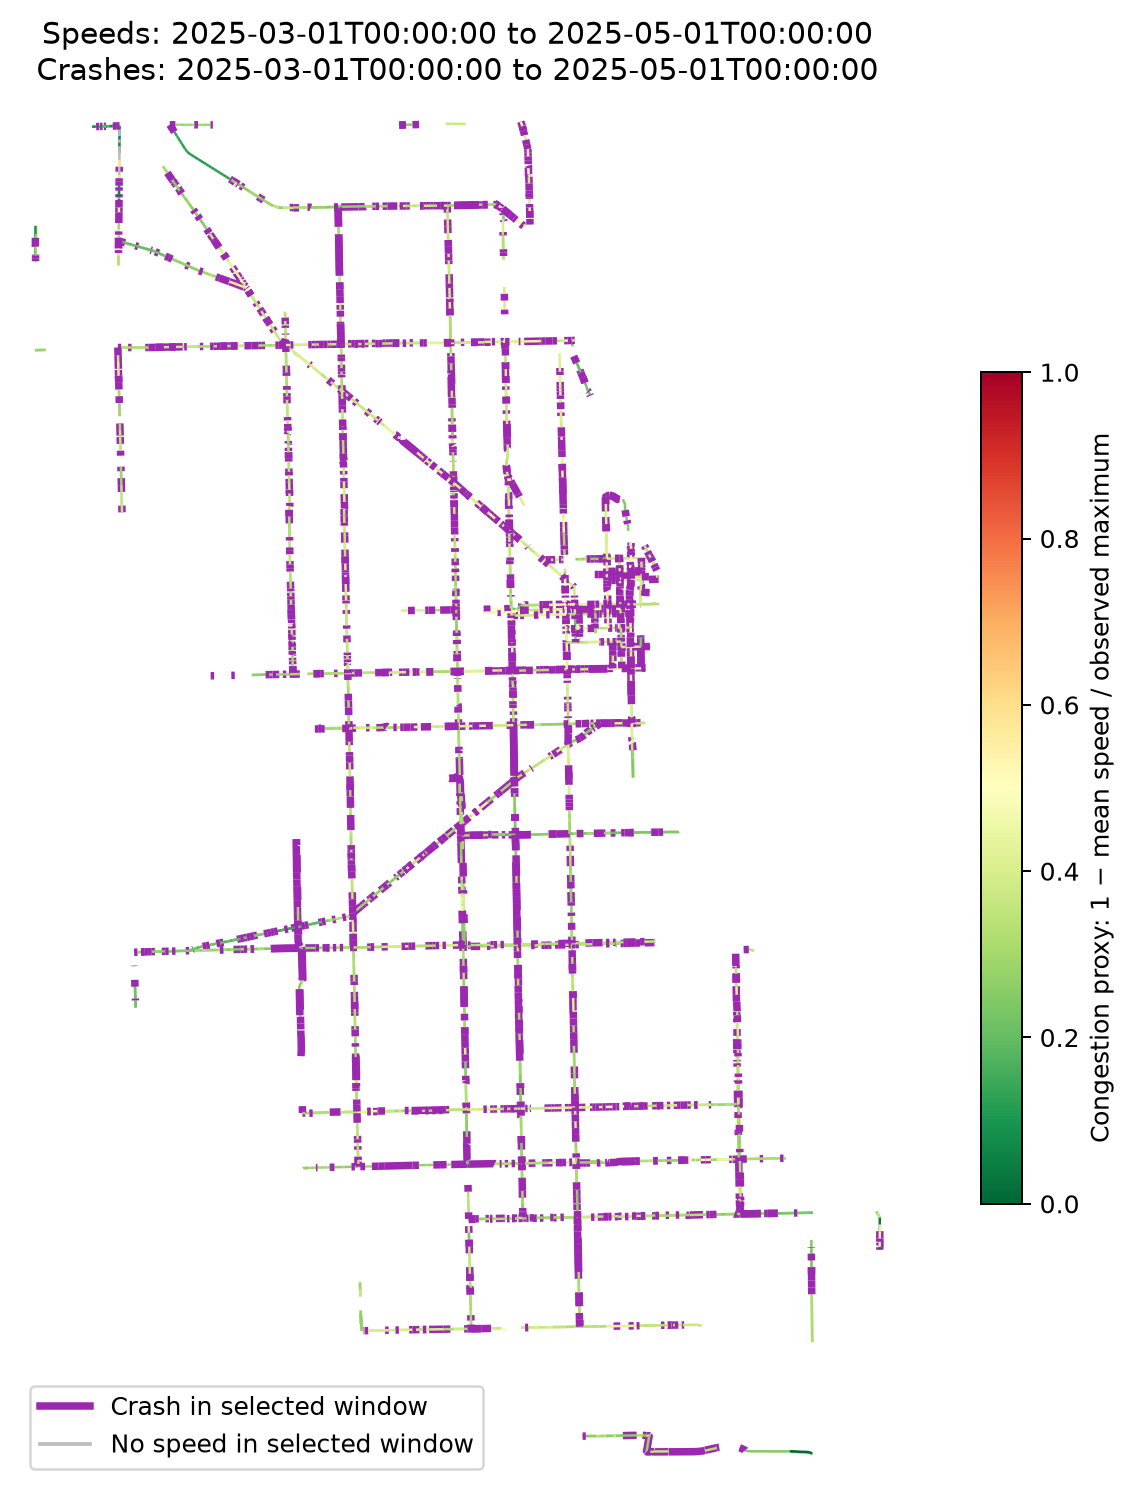
\includegraphics[width=\columnwidth]{road_network.png}%
}{%
  \fbox{\parbox[c][1.30in][c]{0.90\columnwidth}{\centering\small
  Add the project road-network map as
  \texttt{figures/road\_network.png}.}}%
}
\caption{{Road-segment network and matched crash
locations during the pilot study period.}}
\label{fig:midpoint_network}
\end{figure}

{The available neighboring-road data make a spillover
analysis plausible. Of the 2{,}529 events, 2{,}437 (96.4\%) have at
least one one-hop neighbor observed in three or more post-crash bins.
At least one neighbor has a complete post-event trajectory with usable
history for 1{,}459 events (57.7\%) at one hop and 1{,}628 (64.4\%) at
two hops.}

\subsection{{No-Accident Speed Forecasting}}
{We trained an MLP, a GCN, and GraphSAGE on crash-free
target windows, and compared them with historical-mean and persistence
forecasts. All models use pre-window speed histories; the graph models
also use road connections. Training minimizes masked forecasting loss
on observed future speeds. Time-ordered training, validation, and test
splits, separated by a gap, contain 6{,}118, 1{,}296, and 1{,}316
windows, respectively. Test errors cover 3{,}033{,}666 observed targets.}

\begin{table}[t]
\centering
\caption{{Held-out speed forecasting error (mph),
one seed. Lower values are better.}}
\label{tab:midpoint_models}
\footnotesize
{\begin{tabular}{lrr}
\toprule
Model & MAE & RMSE \\
\midrule
GraphSAGE & 3.385 & 4.680 \\
GCN & 3.427 & 4.709 \\
MLP (no edges) & 3.448 & 4.741 \\
Historical mean & 3.546 & 4.873 \\
Persistence & 4.557 & 6.232 \\
\bottomrule
\end{tabular}}
\end{table}

{The learned models improve on the two simple
baselines. However, the controlled GCN--MLP comparison differs by
only 0.022 mph in MAE. GraphSAGE performs best in this run, but it
also has more parameters per layer. These results establish a working
forecasting comparison, not a reliable graph-specific advantage or
evidence of lower causal bias.}

\subsection{{Preliminary Crash-Segment Estimates}}
{We use the GCN to forecast expected speeds without a
crash from pre-event observations. At each horizon, we compare its
prediction residual (observed minus predicted speed) on crash segments
with the same residual in matched crash-free windows that were not used
for model training. This adjustment is intended to reduce forecasting
bias when the controls are comparable:}
\begin{equation}
\widehat{\tau}_h =
\overline{(y-\widehat y^{(0)})}_{\mathrm{crash},h}
-\overline{(y-\widehat y^{(0)})}_{\mathrm{control},h}.
\end{equation}
{The analysis uses 2{,}529 crash events and 4{,}813
matched control windows, with about 1{,}800 observed crash outcomes
per horizon. Figure~\ref{fig:midpoint_effect} shows negative residual
differences at all six horizons. The largest occurs 20--30 minutes
after a crash ($-0.641$ mph; nominal 95\% interval $[-0.94,-0.35]$).
The pooled estimate is about $-0.43$ mph in this run. These results
concern the \emph{crash segment only}; neighboring-road effects have
not yet been estimated.}

\begin{figure}[t]
\centering
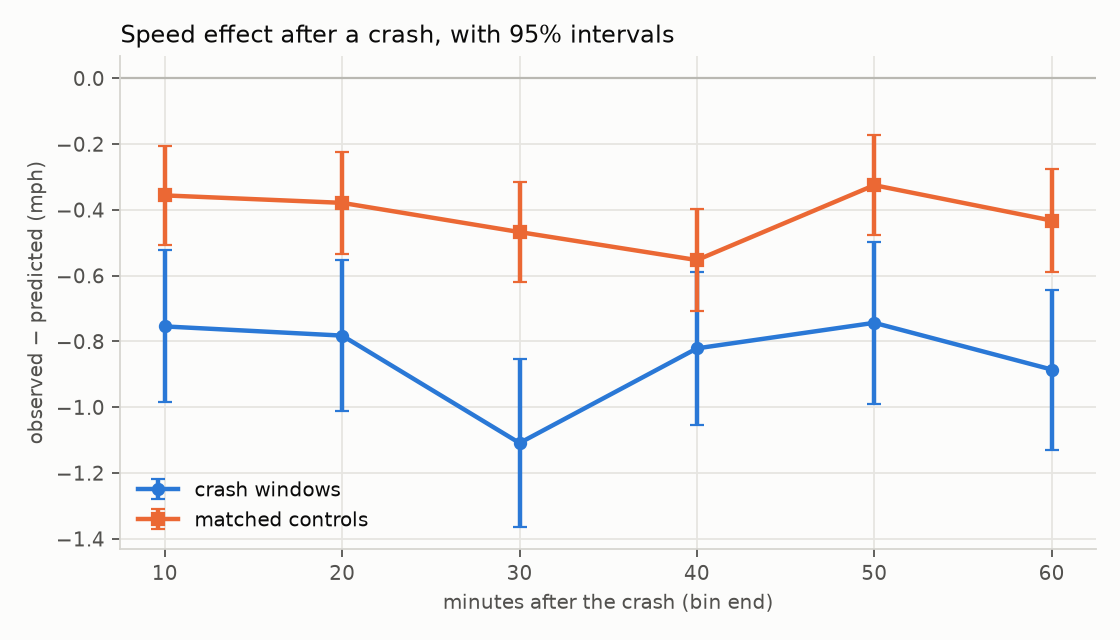
\includegraphics[width=\columnwidth]{crash_effect.png}
\caption{{Crash-minus-control forecast residuals on
crash segments, with nominal 95\% intervals. Negative values indicate
lower speeds relative to matched control conditions.}}
\label{fig:midpoint_effect}
\end{figure}

\subsection{{Limitations and Remaining Work}}
{The findings are preliminary and observational.
Crashes may follow existing congestion, and matched controls cannot
account for every unobserved difference. Estimates also depend on
control selection: across three draws, the pooled result ranged from
about $-0.34$ to $-0.43$ mph. Only 1.9 eligible control windows per
crash were available on average. The reported intervals are nominal,
with no adjustment across six horizons, and models were evaluated with
one seed. We have not yet tested effects on neighboring roads.}

{Our next steps are to extend the study period and
improve control selection; train a spatiotemporal GNN; and evaluate
counterfactual effect recovery using semi-synthetic disruptions with
known effects. We will then compare direct and neighboring-road
estimates, test the contribution of graph structure, and examine
pre-event trends, placebo events, and uncertainty.}
% END MIDPOINT ADDITION

\section{Study Scope and Causal Targets}
\textbf{Event definition.} We will start with crashes located on
monitored arterial segments and recorded within the available speed
history. A crash will serve as the event for a short before-and-after
window. We will check whether it can be located on a unique directed
segment and whether there are usable observations on its neighbors.

\textbf{Effects of interest.} We will distinguish the speed change on
the crash segment from changes on connected segments. Candidate
horizons are ten-minute steps in roughly the first hour after an event;
we may extend the window where coverage permits. We will report
both the size and duration of slowdowns, including differences between
upstream and downstream segments if directions can be resolved.

\textbf{Counterfactual.} For each exposed segment, the target is the
speed expected at the same time had the reported crash not occurred.
This outcome cannot be observed directly. Our estimates will depend
on matched crash-free periods and models fitted without information
from after the crash in the event being evaluated.

\section{Research Questions}
\begin{itemize}
    \item How do accident-related slowdowns vary across connected
    roads and time after an event?
    \item Does graph learning improve counterfactual estimation
    compared with methods that ignore road connections?
    \item Do direction, distance, or network position help explain
    which segments experience larger or longer effects?
\end{itemize}

\section{Proposed Approach}
\subsection{Causal Design}
We will match accident periods with crash-free periods on the same or
comparable roads. Matching will use hour, day, season, and traffic
conditions observed \emph{before} the event. A matched event study
will estimate changes relative to these controls. Depending on overlap
and sample size, we may add outcome regression or doubly robust
adjustment.

We will define direct and neighboring exposure before examining the
post-accident outcomes. Periods with other nearby reported crashes
will be excluded or flagged. We will compare pre-event speed trends
and require sufficient overlap between crash and control periods.
The causal interpretation rests on the assumption that selected
controls approximate the speeds that would have occurred without the
crash. This adjusts for observed congestion, not every hidden cause.

\subsection{Graph Machine Learning}
We will test message-passing or spatiotemporal graph models that use
road connectivity and pre-event speed histories. Models may estimate
the expected no-accident speed or learn representations for estimating
direct and neighboring effects. Network interference motivates this
approach \cite{ma2021interference}; a graph convolutional network is
one possible baseline \cite{kipf2017gcn}.

The initial graph will use verified road connections. Edge direction,
network distance, and centrality can be added where useful. One
candidate combines spatial message passing with a small temporal
encoder over pre-event speeds. This could capture both road structure
and the recent traffic trend without requiring a new architecture.
We will not treat correlated speeds as proof of causal edges, and we
will not use post-event measurements as counterfactual inputs.

\subsection{Model Comparison}
We will compare (i) a matched event-study baseline, (ii) a non-graph
causal or outcome model, and (iii) a graph-aware model. Models will use comparable pre-event inputs. The non-graph model will
also receive simple summaries of neighboring speeds, so a GNN must
add value beyond access to neighbor data. Ablations will remove road
links or neighbor features to test the contribution of graph learning.

\section{Identification and Evaluation}
\textbf{Assumptions.} Control periods must provide credible untreated
trends, and the graph must capture the main roads exposed to each
event. Accidents are not random: congestion may increase crash risk.
Approximate reporting times, missing speeds, and other incidents can
also bias estimates.

\textbf{Causal checks.} We will examine pre-event trends, placebo
event times, different matching rules, and alternate exposure
neighborhoods. Effects will be reported by time since the accident
and network distance, with uncertainty grouped by accident event.
We will report the fraction of events with complete speed coverage.

\textbf{GML checks.} We will test on held-out events and time periods,
keeping observations from the same event together. Prediction error
on crash-free periods will be reported separately from causal
robustness. If feasible, semi-synthetic effects on the real road graph
will give a benchmark with known counterfactual outcomes.

\section{Experimental Plan}
\textbf{Data construction.} Match crash reports to road geometry and
speed observations. Exclude uncertain matches and record missing
values; do not treat missing speed as zero. Build before-and-after
event windows on the ten-minute time grid.

\textbf{Exposure and controls.} Begin with the crash segment and
immediately connected roads. Compare upstream and downstream effects
if direction is reliable. Select crash-free controls using pre-event
conditions, and verify their speed trends before treatment.

\textbf{Learning and testing.} Train graph and non-graph estimators on
comparable data splits. Compare estimated effects, lead-time placebos,
uncertainty, and sensitivity to removing road connections. A better
speed predictor will not automatically count as a better causal model.

\section{Research Tests and Success Criteria}
\textbf{Primary test.} Compare estimated slowdowns on the incident
segment and its one- and two-hop neighbors, with uncertainty bands.
A result that varies systematically across road direction or graph
distance would provide an interpretable network finding, even if
complex models offer no improvement.

\textbf{Model contribution.} Compare the graph model with a temporal
model using the same pre-event observations and a baseline that also
receives simple neighboring-speed summaries. Test a graph with removed
or rewired edges to distinguish useful road structure from added model
capacity. We will not call lower prediction error evidence of lower
causal bias without further tests.

\textbf{Known-effect check.} If feasible, inject simulated speed
shocks into real, crash-free histories on the observed road graph. The
shock size, direction, and propagation pattern will be known, so we
can measure error in recovered effects and interval coverage. Such
tests support method evaluation but cannot validate causal assumptions
for actual crashes.

{\textbf{Midpoint update:} We are prioritizing this
benchmark in the remaining study. It will test how accurately the
models recover known effects, separately from forecasting accuracy.}

\textbf{Feasibility threshold.} The pilot must show enough events with
reliable crash-to-segment matches, valid pre/post speeds, and candidate
controls. If neighboring coverage is weak, we will narrow the study
to well-observed corridors rather than impute large portions of the
network or claim unsupported spillovers.

{\textbf{Midpoint finding:} Network connectivity
and neighboring-road observation counts support proceeding with
spillover experiments. They do not yet establish that effects can be
identified reliably.}

\section{Potential Extensions}
\begin{itemize}
    \item \textbf{Dynamic propagation:} Study how upstream and
    downstream effects evolve with spatiotemporal GNNs.
    \item \textbf{Heterogeneous effects:} Test variation by crash type,
    time of day, and road centrality.
    \item \textbf{Robust causal learning:} Explore latent traffic
    conditions, geographic transfer, and semi-synthetic benchmarks.
    \item \textbf{Network vulnerability:} Identify road segments
    associated with larger spillovers, if causal estimates are credible.
\end{itemize}

\section{Hypotheses and Interpretation}
\textbf{H1: Network exposure matters.} We expect the average
accident-related speed reduction to be greatest near the incident,
with possible differences between upstream and downstream segments.
We will test this pattern rather than impose it as a model assumption.
A negligible neighboring effect is also a meaningful result.

\textbf{H2: Graph learning adds information.} When road connections
are informative, a graph model may estimate untreated speeds more
accurately than a temporal model alone. The stronger claim---that it
recovers causal effects more reliably---will be tested with placebo
checks and, if feasible, known-effect simulations. We will distinguish
these two claims in every result table.

\textbf{Scope of claims.} Even a consistent effect pattern does not
prove that congestion physically traveled along each graph edge.
Changes in route choice, traffic signals, and common demand shocks
can create similar patterns. We will describe the estimated effects
as conditional on our matched-control design rather than assert
that the GNN discovered a causal road network.

\section{Reproducibility and Deliverables}
We plan to release code for event matching, road-graph construction,
data-quality reports, model training, and causal diagnostics. Scripts
will retain the exact sample filters and train/test event assignments.
The report will include a coverage map, an event-time plot for direct
and neighboring roads, an ablation table, and an explanation of cases
where the causal assumptions appear weak. We will also report the
runtime and data requirements of the main models. This makes the
project useful even if a complex model does not outperform the
simpler causal baseline.

\section{Expected Outcome and Plan}
\textbf{Stage 1:} Validate crash matching, traffic coverage, and graph
connections. \textbf{Stage 2:} Construct matched events and estimate
baseline direct and neighboring effects. \textbf{Stage 3:} Train graph
models and run network ablations. \textbf{Stage 4:} Test causal
assumptions, uncertainty, and one extension supported by the data.

We expect a reproducible study of whether, when, and how network
learning improves estimates of crash-related congestion. Weak or null
graph effects will also be reported.

{\textbf{Status at midpoint:} Data integration,
road-graph construction, baseline training, and an initial direct-effect
analysis are complete. Spatiotemporal training, semi-synthetic
validation, spillover estimation, and robustness checks remain for the
final report.}

\bibliographystyle{template/ACM-Reference-Format}
\bibliography{proposal}
\end{document}
